\chapter{Información General del Proyecto}

Este capítulo describe la ubicación del proyecto, la caracterización eléctrica del circuito 10-502, el punto de conexión propuesto y los parámetros técnicos de los equipos de generación y transformación. La información aquí consolidada constituye la base sobre la cual se construyen los análisis de los capítulos posteriores.

\section{Ubicación Geográfica y Fecha de Entrada en Operación}

El proyecto se localiza en Bucaramanga, departamento de Santander, sobre la Carrera~34, en las instalaciones del supermercado MAS~X~MENOS sede Guarín. La entrada en operación se proyecta para el año 2025. Las coordenadas geográficas del predio se presentan en la Tabla~\ref{tab:coords} y su localización relativa se ilustra en la Figura~\ref{fig:localizacion}.

\begin{table}[H]
    \centering
    \caption{Coordenadas ubicación geográfica del proyecto}
    \label{tab:coords}
    \begin{tabular}{cc}
    \toprule
    \textbf{Latitud} & \textbf{Longitud} \\
    \midrule
    7,12621563 & $-$73,11227598 \\
    \bottomrule
    \end{tabular}
\end{table}

\begin{figure}[H]
    \centering
    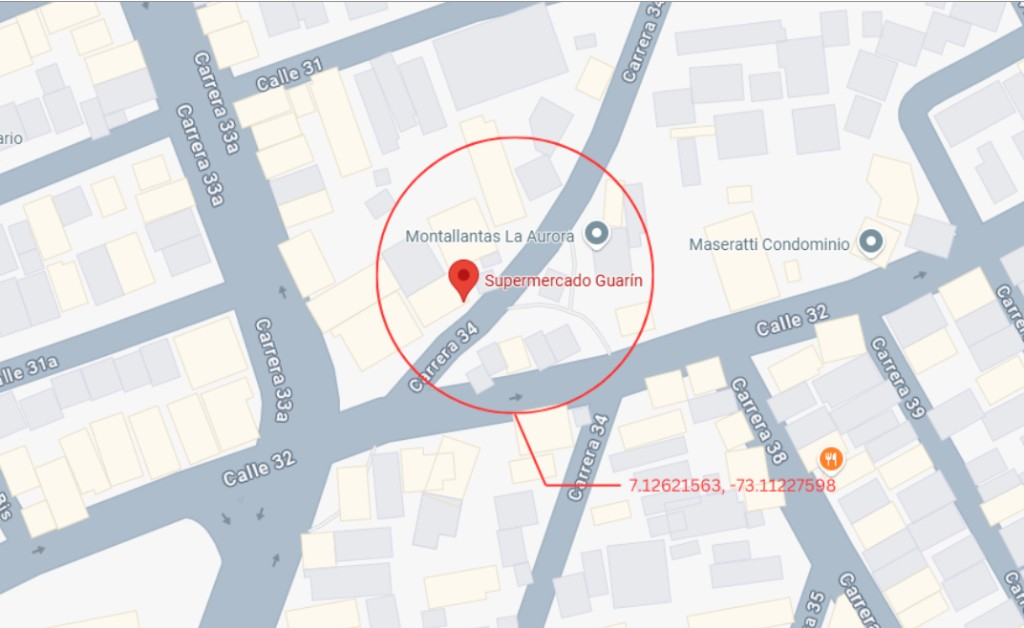
\includegraphics[width=0.95\textwidth]{figuras/figura1_localizacion.png}
    \caption{Localización del proyecto}
    \label{fig:localizacion}
\end{figure}

\section{Caracterización del Circuito 10-502}

La red de conexión corresponde al circuito \textbf{10-502} de la subestación Conucos, operado a 13,8~kV según la información entregada por ESSA. El modelo eléctrico construido a partir de esos datos incluye 215 tramos de línea, con una longitud total modelada de 5,061~km, y 51 cargas en baja tensión cuya suma asciende a 7,532~MVA. La demanda máxima registrada en cabecera es de 1,683~MVA a las 12:00~h, equivalente a una corriente de 70,41~A, mientras que la demanda mínima del día se sitúa en 0,630~MVA a las 04:00~h. El punto de conexión del AGPE es el nodo 3272966. Estos parámetros se consolidan en la Tabla~\ref{tab:resumen_cto}.

\begin{table}[H]
    \centering
    \caption{Resumen del modelo eléctrico del circuito 10-502}
    \label{tab:resumen_cto}
    \begin{tabular}{lc}
    \toprule
    \textbf{Parámetro} & \textbf{Valor} \\
    \midrule
    Subestación / campo & SE Conucos / 10-502 \\
    Tensión nominal & 13,8 kV \\
    Número de tramos de línea & 215 \\
    Longitud total modelada & 5,061 km \\
    Número de cargas LV & 51 \\
    Suma de cargas modeladas & 7,532 MVA \\
    Demanda máxima en cabecera & 1,683 MVA (12:00 h) \\
    Corriente máxima en cabecera & 70,41 A \\
    Demanda mínima en cabecera & 0,630 MVA (04:00 h) \\
    Punto de conexión AGPE & Nodo 3272966 \\
    \bottomrule
    \end{tabular}
\end{table}

El perfil horario de demanda del 19/03/2024, mostrado en la Figura~\ref{fig:demanda}, evidencia un comportamiento típico de un alimentador con carga comercial e institucional: valle nocturno, rampa matutina y pico cercano al mediodía. Sobre esa base se seleccionaron las tres horas de análisis reportadas en la Tabla~\ref{tab:demanda_horas}, que cubren la franja matutina, el máximo diario y la operación vespertina.

\begin{figure}[H]
    \centering
    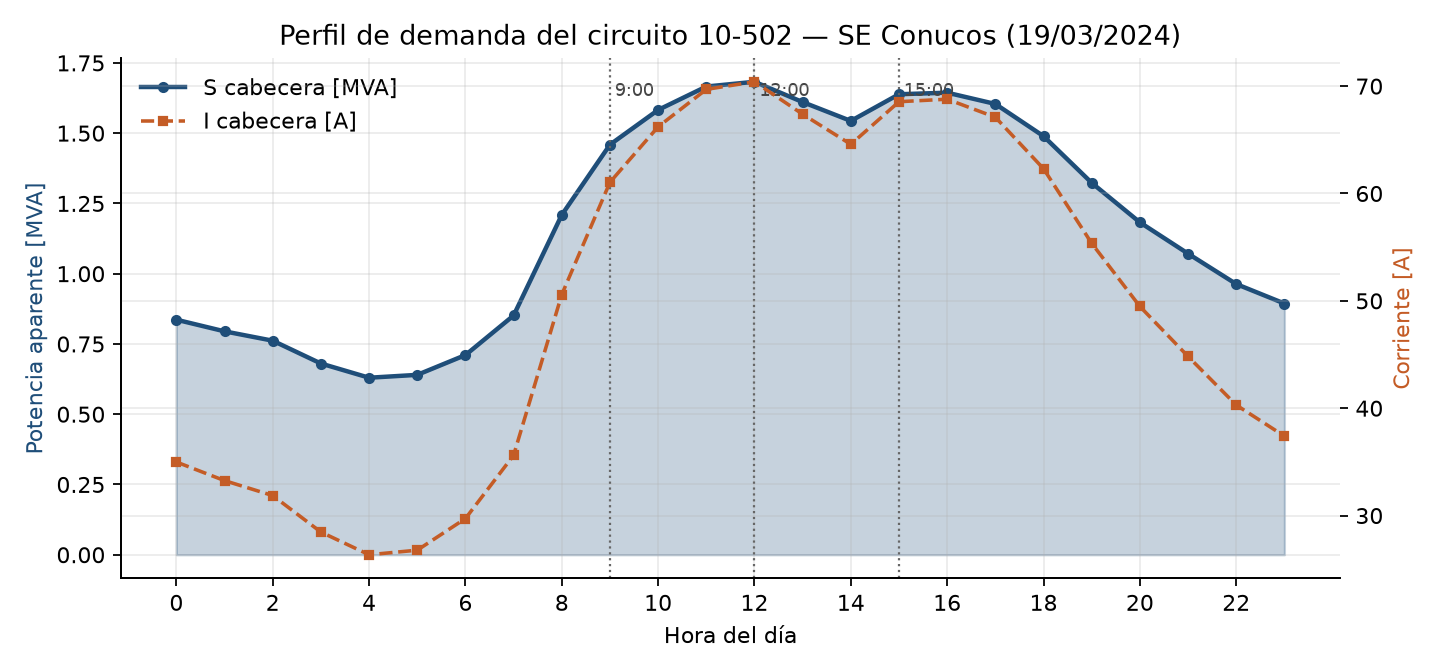
\includegraphics[width=0.95\textwidth]{figuras/fig_demanda_circuito.png}
    \caption{Perfil horario de demanda del circuito 10-502 (19/03/2024)}
    \label{fig:demanda}
\end{figure}

\begin{table}[H]
    \centering
    \caption{Demanda en cabecera del circuito en las horas de análisis}
    \label{tab:demanda_horas}
    \begin{tabular}{cccc}
    \toprule
    \textbf{Hora} & \textbf{I [A]} & \textbf{S [MVA]} & \textbf{Observación} \\
    \midrule
    09:00 & 61,05 & 1,459 & Franja matutina \\
    12:00 & 70,41 & 1,683 & Demanda máxima del día \\
    15:00 & 68,55 & 1,638 & Franja vespertina \\
    \bottomrule
    \end{tabular}
\end{table}

La composición de conductores del circuito, ilustrada en la Figura~\ref{fig:conductores}, refleja una red predominantemente en cable de cobre XLPE de distintos calibres, coherente con un alimentador urbano de media tensión. Por su parte, la Figura~\ref{fig:topcargas} identifica las principales cargas modeladas y resalta la carga asociada al punto de conexión, lo que permite ubicar el proyecto dentro del contexto de demanda del alimentador.

\begin{figure}[H]
    \centering
    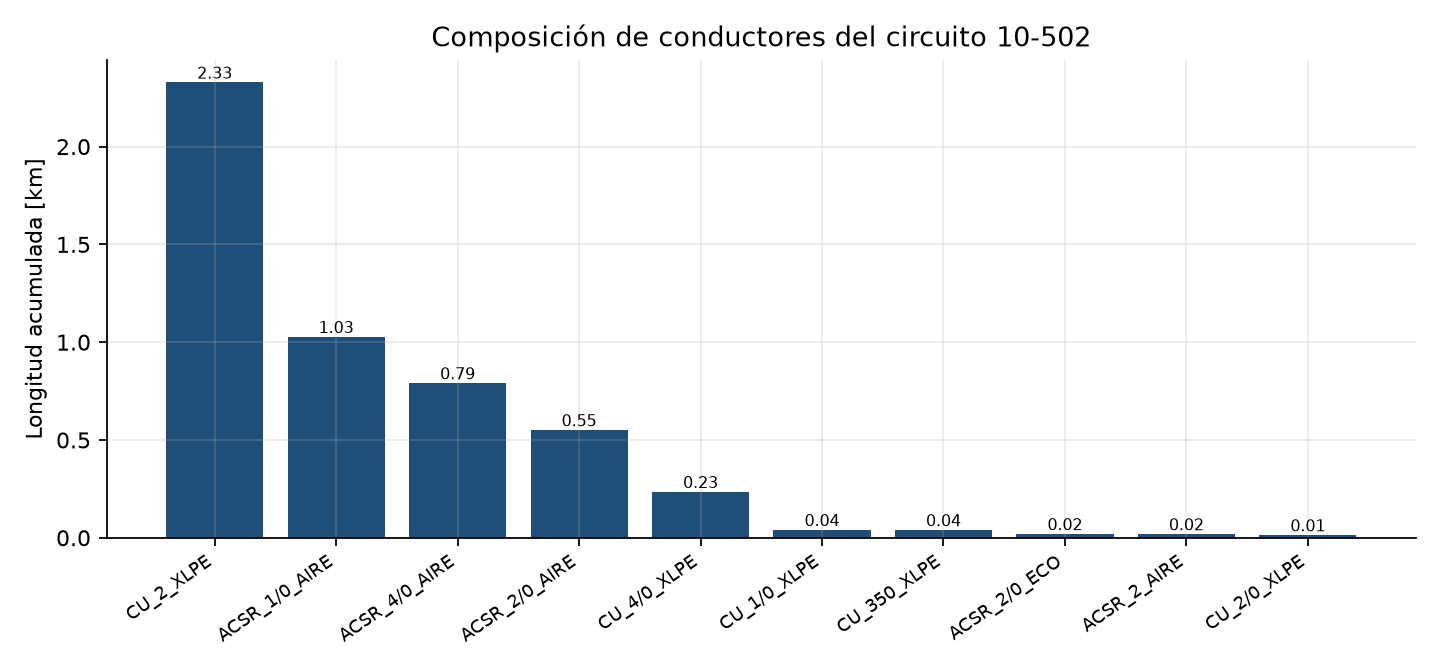
\includegraphics[width=0.95\textwidth]{figuras/fig_conductores.png}
    \caption{Composición de conductores del circuito 10-502}
    \label{fig:conductores}
\end{figure}

\begin{figure}[H]
    \centering
    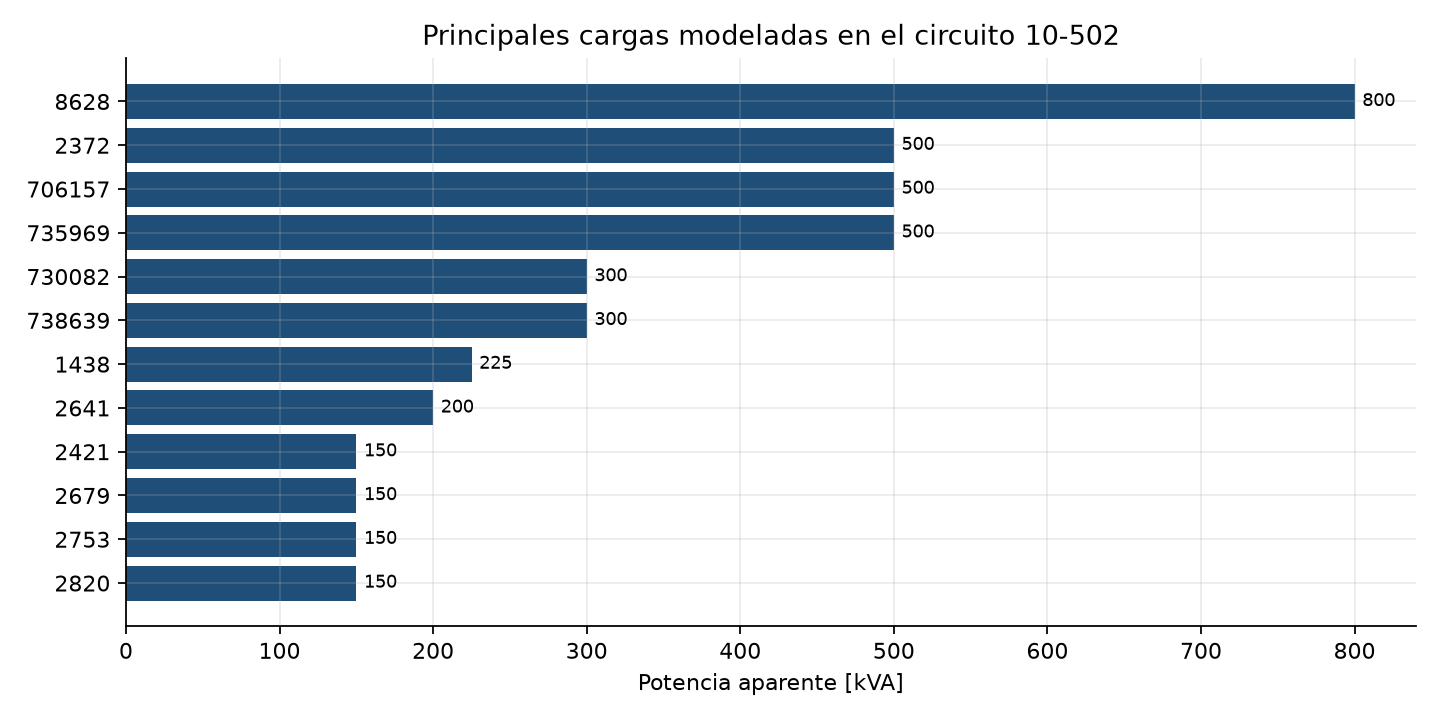
\includegraphics[width=0.95\textwidth]{figuras/fig_top_cargas.png}
    \caption{Principales cargas modeladas (resaltada la carga del POC 3272966)}
    \label{fig:topcargas}
\end{figure}

\section{Parámetros Técnicos del Nodo 3272966}

El apoyo o nodo de conexión del AGPE es el \textbf{3272966}. Los parámetros eléctricos de las líneas en el SDL fueron suministrados por el operador de red y fueron los utilizados para modelar el sistema de distribución de ESSA, así como el equivalente de red en la subestación Conucos, conforme al estudio \textit{SUB\_EST\_CONEX\_MAS\_X\_MENOS\_GUARIN}.

El transformador utilizado para la conexión del proyecto a la red se modeló con los parámetros de la Tabla~\ref{tab:trafo}. Las características de la línea de conexión en media tensión se presentan en la Tabla~\ref{tab:linea_conexion}. El conductor propuesto es el mismo utilizado para alimentar la demanda en el nodo 3272966: cable CU~2~XLPE.

\begin{table}[H]
    \centering
    \caption{Parámetros técnicos del transformador Serie 21123832-S 13,2 kV/220 V}
    \label{tab:trafo}
    \begin{tabular}{lcc}
    \toprule
    \textbf{Parámetro} & \textbf{Valor} & \textbf{Unidad} \\
    \midrule
    Potencia & 150 & kVA \\
    Tensión primario / secundario & 13,2 / 220 & kV / V \\
    Impedancia de cortocircuito ($Z_{cc}$) & 4,9 & \% \\
    Grupo de conexión & Dyn5 & -- \\
    \bottomrule
    \end{tabular}
\end{table}

\begin{table}[H]
    \centering
    \caption{Característica de la línea de conexión del transformador ESSA Serie 21123832-S 13,2 kV}
    \label{tab:linea_conexion}
    \begin{tabular}{lc}
    \toprule
    \textbf{Parámetro} & \textbf{Valor} \\
    \midrule
    Línea & 3272869 -- 3272966 \\
    Número de circuitos & 1 \\
    Conductor & Cable CU 2 XLPE \\
    $R'_1$ (AC, 20~°C) & 0,0020 $\Omega$ \\
    $X'_1$ & 0,0013 $\Omega$ \\
    $R'_{0}$ (AC) & 0,0033 $\Omega$ \\
    $X'_{0}$ & 0,0012 $\Omega$ \\
    \bottomrule
    \end{tabular}
\end{table}

\begin{figure}[H]
    \centering
    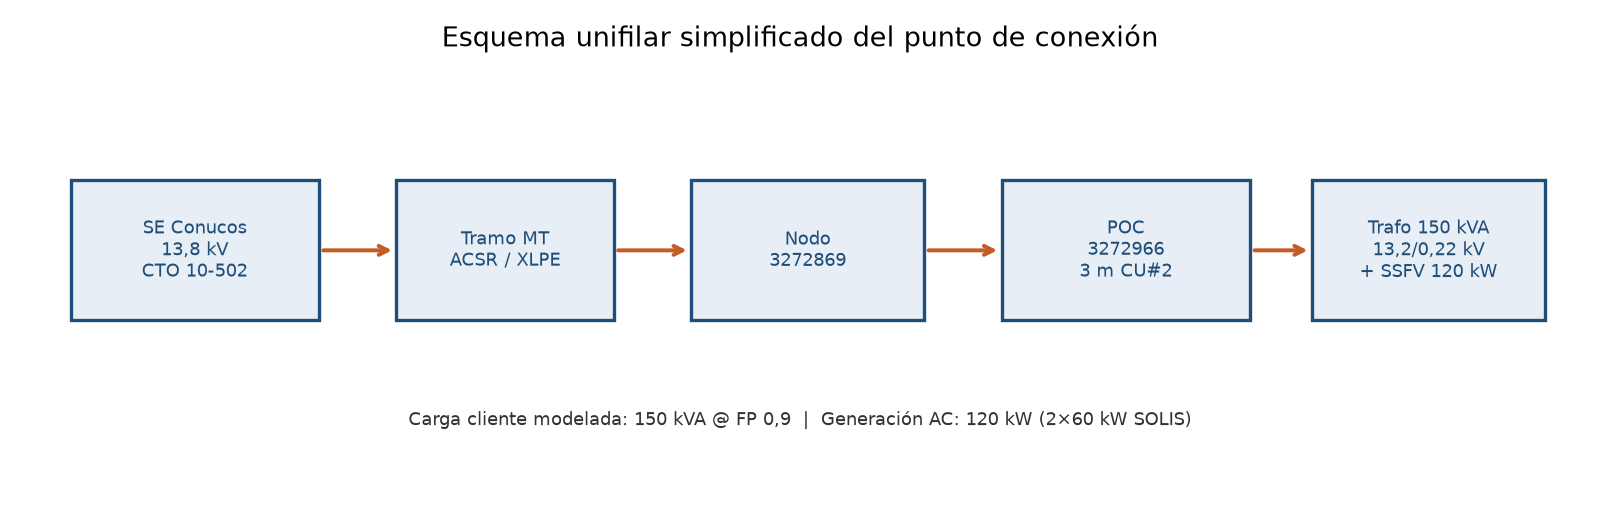
\includegraphics[width=\textwidth]{figuras/fig_esquema_poc.png}
    \caption{Esquema unifilar simplificado del punto de conexión}
    \label{fig:esquema}
\end{figure}

\section{Parámetros Técnicos de Inversores y Paneles}

La planta fotovoltaica se configura a partir de dos bloques de conversión y un arreglo de módulos de alta eficiencia. A continuación se detallan las especificaciones relevantes para el modelado eléctrico y para la estimación de producción energética.

\subsection{Inversores}

Se instalarán dos inversores SOLIS~60K-LV-5G, cada uno con potencia máxima de 69~kW, tensión nominal de salida de 220~VAC y frecuencia de 60~Hz. El equipo opera a tres fases, incorpora protección anti-isla y trabaja con factor de potencia de 0,99. El rango MPPT de entrada en corriente continua se extiende entre 180 y 1000~VDC, con una tensión máxima de 1100~VDC. La Tabla~\ref{tab:inversores} resume estos parámetros.

\begin{table}[H]
    \centering
    \caption{Parámetros técnicos del inversor SOLIS 60K LV 5G}
    \label{tab:inversores}
    \begin{tabular}{lcc}
    \toprule
    \textbf{Parámetro} & \textbf{Valor} & \textbf{Unidad} \\
    \midrule
    Número de inversores & 2 & UND \\
    Tensión máxima de arranque & 195 & VDC \\
    Tensión MPPT en DC entrada & 180 -- 1000 & VDC \\
    Tensión máxima DC entrada & 1100 & VDC \\
    Máxima corriente de entrada & $26 \times 8$ & A DC \\
    Potencia máxima & 69000 & W \\
    Voltaje nominal de salida & 220 & VAC \\
    Frecuencia de salida & 60 & Hz \\
    Corriente de salida & 157,5 & A \\
    Número de fases & 3 & -- \\
    Protección anti-isla & Sí & -- \\
    Factor de potencia & 0,99 & -- \\
    \bottomrule
    \end{tabular}
\end{table}

\subsection{Paneles Fotovoltaicos}

El campo solar estará compuesto por 240 paneles JINKO monocristalinos mono-faciales de 590~W cada uno, con voltaje máximo de salida de 41,05~VDC, corriente máxima de 10,83~A y eficiencia de 22,84\%. La Tabla~\ref{tab:paneles} consolida estas especificaciones. La Figura~\ref{fig:genvsdem} contrasta el perfil estimado de generación fotovoltaica con la demanda del cliente en el punto de conexión, evidenciando el potencial de autoconsumo durante las horas de mayor irradiación.

\begin{table}[H]
    \centering
    \caption{Parámetros técnicos de los paneles fotovoltaicos}
    \label{tab:paneles}
    \begin{tabular}{lcc}
    \toprule
    \textbf{Parámetro} & \textbf{Valor} & \textbf{Unidad} \\
    \midrule
    Tipo & \multicolumn{2}{l}{JINKO Monocristalino Mono-facial} \\
    Potencia nominal por panel & 590 & W \\
    Voltaje máximo de salida & 41,05 & VDC \\
    Corriente máxima de salida & 10,83 & A \\
    Eficiencia & 22,84 & \% \\
    Cantidad de paneles & 240 & UND \\
    \bottomrule
    \end{tabular}
\end{table}

\begin{figure}[H]
    \centering
    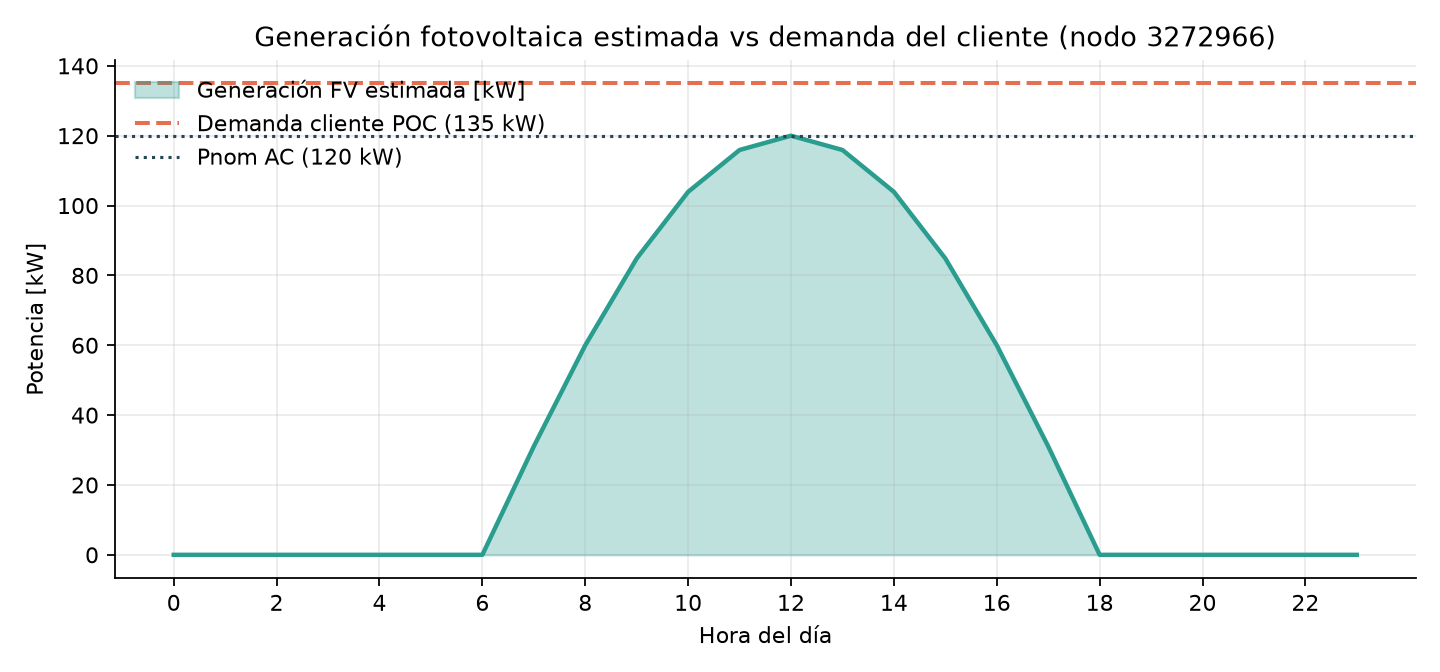
\includegraphics[width=0.95\textwidth]{figuras/fig_gen_vs_demanda.png}
    \caption{Perfil estimado de generación FV vs demanda del cliente en el POC}
    \label{fig:genvsdem}
\end{figure}

\section{Cálculo de Energía Producida}

La estimación de energía anual permite dimensionar el beneficio energético del proyecto y contrastarlo con la demanda local. Para ello se combinan el recurso solar del sitio, la configuración geométrica del arreglo y las pérdidas típicas del sistema.

\subsection{Radiación Solar}

La radiación global anual promedio sobre superficie horizontal en Bucaramanga se estima en 4,7~kWh/m$^2$/día, valor representativo de la zona andina oriental y suficiente para sostener una producción atractiva con módulos de alta eficiencia.

\subsection{Ausencia de Sombras}

En la planta proyectada no se identifica sombreado significativo que afecte de manera relevante la generación del sistema fotovoltaico. En consecuencia, las pérdidas por sombreado se consideran nulas en el balance energético.

\subsection{Datos de Entrada}

Los datos de entrada para el cálculo de energía se resumen en la Tabla~\ref{tab:energia_in}. Incluyen la capacidad instalada, la orientación e inclinación del arreglo, las pérdidas globales del sistema (26\%) y la eficiencia del inversor (98,50\%), con una relación DC/AC de 1,18.

\begin{table}[H]
    \centering
    \caption{Datos de entrada para estimar la energía generada}
    \label{tab:energia_in}
    \begin{tabular}{lc}
    \toprule
    \textbf{Parámetro} & \textbf{Valor} \\
    \midrule
    Ubicación del proyecto & Bucaramanga \\
    Coordenadas (LAT, LONG) & 7,12621563, $-$73,11227598 \\
    Capacidad instalada en DC & 141,6 kWp \\
    Capacidad instalada en AC & 120 kW \\
    Tipo de módulo & Premium \\
    Inclinación & 10° \\
    Azimut & 180 \\
    Pérdidas del sistema & 26\% \\
    Eficiencia del inversor & 98,50\% \\
    Relación DC a AC & 1,18 \\
    \bottomrule
    \end{tabular}
\end{table}

\subsection{Fórmula de Energía Producida}

La energía anual estimada se calcula mediante la expresión:

\begin{equation}
E_{p,y} = P_{nom}(d.c) \times Irr \times (1 - \text{Losses})
\end{equation}

donde $P_{nom}(d.c)=141,6$~kWp es la potencia nominal en corriente continua, $Irr=1.715,5$~kWh/m$^2$/año es la irradiación anual equivalente sobre el plano de los módulos y $\text{Losses}=26\%$ concentra las pérdidas del sistema. Con estos parámetros se obtiene una producción estimada del orden de \textbf{179.757~kWh/año}.

\section{Equivalente de Red en SE Conucos}

Para el análisis de cortocircuito se emplea el equivalente de red en el barraje de 13,8~kV de la subestación Conucos, reportado por el operador. La Tabla~\ref{tab:sc_conucos} presenta los niveles de falla trifásica y monofásica a tierra, junto con la relación R/X asociada. Estos valores definen la contribución de la red aguas arriba y constituyen el principal aporte de corriente de cortocircuito en el alimentador.

\begin{table}[H]
    \centering
    \caption{Niveles de falla en barraje 13,8 kV -- S/E Conucos}
    \label{tab:sc_conucos}
    \begin{tabular}{lcccc}
    \toprule
    \textbf{Tipo de falla} & \textbf{$S_k$ [MVA]} & \textbf{$I_k$ [kA]} & \textbf{$I_p$ [kA]} & \textbf{R/X} \\
    \midrule
    Trifásica & 654,488 & 27,382 & 70,401 & 0,068 \\
    Monofásica a tierra & 239,681 & 30,083 & 77,345 & 0,068 \\
    \bottomrule
    \end{tabular}
\end{table}

\section{Protección Existente del Circuito}

Según la hoja de protecciones del operador, la bahía del circuito 10-502 dispone de un relé AREVA MICOM~P142 como protección principal de sobrecorriente, con funciones 50, 50N, 51 y 51N. El equipo opera a 13,8~kV con relaciones de transformación de corriente y potencial RTC/RTP de 60/120. Los ajustes de fase y tierra, así como la lógica de recierre, se detallan en la Tabla~\ref{tab:rele_existente}. Estos parámetros serán contrastados, más adelante, con el aporte del AGPE y con las protecciones del lado de baja tensión del proyecto.

\begin{table}[H]
    \centering
    \small
    \caption{Protección principal del circuito 10-502 (SE Conucos)}
    \label{tab:rele_existente}
    \begin{tabular}{ll}
    \toprule
    \textbf{Parámetro} & \textbf{Valor} \\
    \midrule
    Subestación / bahía & Conuco / CTO 10502 \\
    Tensión & 13,8 kV \\
    RTC / RTP & 60 / 120 \\
    Fabricante / modelo & AREVA / MICOM P142 \\
    Serial & 360 \\
    Funciones & 50, 50N, 51, 51N \\
    Tipo & Protección principal de sobrecorriente \\
    51 (fase) & Pickup 6, dial 0,1, curva IEC VI \\
    50-1 (fase) & Pickup 36, retardo 0 s \\
    51N (tierra) & Pickup 2, dial 0,15, curva IEC VI \\
    50N & Pickup 20 \\
    Recierre 79 & 15/30 s, reset 60 s \\
    \bottomrule
    \end{tabular}
\end{table}
